\begin{homeworkProblem}
What is the Poynting vector $\mathbf{S}(R, \theta)$ in a spherical coordinate frame whose center is at the current time (t) location of a charge moving at constant velocity. How does this vary with $R$? What is $\mathbf{S}$ for $\theta = 0$ and $\theta = 90^\circ$? See pages 461–462 of the text.
\begin{callout}{Solution:}

    A moving charge in polar coordinates has fields
    \begin{align*}
            \mathbf{E}(\mathbf{r}, t) &= \frac{q}{4\pi \epsilon_{0}} \frac{1-v^{2} / c^{2}}{(1-v^{2}\sin^{2} \theta / c^{2})^{\frac{3}{2}}} \frac{\mathbf{\hat{R}}}{R^{2}} \tag{10.75} \\ 
            \mathbf{B} &= \frac{1}{c^{2}} (\mathbf{v}\times \mathbf{E}) \tag{10.76}
    \end{align*}

    The cross product between the two is needed:
    \begin{align*}
        \mathbf{E\times B} &= \frac{1}{c^{2}} \mathbf{E} \times \mathbf{v} \times \mathbf{E} \\ 
        &= \frac{1}{c^{2}} \left[ \mathbf{v}(\mathbf{E}\cdot \mathbf{E}) - \mathbf{E}(\mathbf{v}\cdot \mathbf{E}) \right] &&\text{(Triple Product Identity)} \\ 
        &= \frac{E^{2}}{c^{2}} \left[ \mathbf{v} - \mathbf{R}v\cos\theta \right]
    \end{align*}
    Therefore, 
    $$\mathbf{S}(\mathbf{R}, \theta) = \frac{E^{2}}{\mu_{0} c^{2}} \left[ \mathbf{v} - \mathbf{R}v\cos\theta \right] = \left( \frac{q}{4\pi \epsilon_{0} R^{2}} \frac{1-v^{2} / c^{2}}{(1-v^{2}\sin^{2} \theta / c^{2})^{3 / 2}} \right)^{2} \frac{1}{\mu_{0}c^{2}}\left[ \mathbf{v} - \mathbf{R}v\cos\theta \right] $$
    In this case, $\mathbf{S}\propto \frac{1}{R^{4}}$. The plot of the function's angular dependence goes as $\sec(\theta)$, and therefore has minima at $\left\{ 0, 180^\circ, 360^\circ, \dots \right\}$. Maxima occur at $\left\{ 0, 90^\circ, 270^\circ, \dots \right\}$.Specifically, at $0^\circ$ and $90^\circ$, $\mathbf{S}=0$ and $\mathbf{S}=\infty$, respectively.


    \begin{centering}
        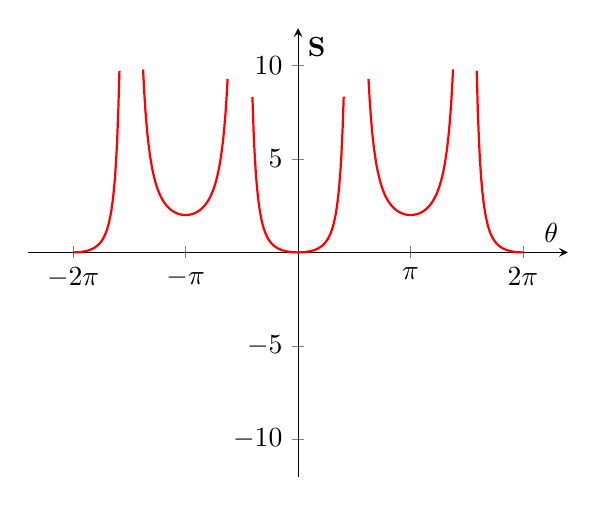
\begin{tikzpicture}
        \begin{axis}[
                domain=-6.28:6.28, % -2π to 2π
                samples=400,
                ymin=-10, ymax=10,
                axis lines=middle,
                xlabel=$\theta$, ylabel={$\mathbf{S}$},
                restrict y to domain=-10:10,
                enlargelimits=true,
                xtick={-6.28, -3.14, 0, 3.14, 6.28},
                xticklabels={$-2\pi$, $-\pi$, $0$, $\pi$, $2\pi$},
                unbounded coords=jump
                ]
                \addplot[red, thick] {(1 - cos(deg(x))) / (cos(deg(x))^2)};
        \end{axis}
    \end{tikzpicture}

    \end{centering}


\end{callout}
\end{homeworkProblem}

\begin{homeworkProblem}
A small dipole has a dipole moment as a function of time:

\[
\mathbf{p}(t') = p_0 \exp\left(-\left(\frac{t'}{\tau}\right)^2\right) \hat{\mathbf{z}}
\]

where $\tau$ is a time constant.

\begin{itemize}
    \item[(a)] Sketch the function $\mathbf{p}(t')$ versus $t'/\tau$. It is a Gaussian centered at $t' = 0$.
        \begin{callout}{Solution:}

            \begin{center}
                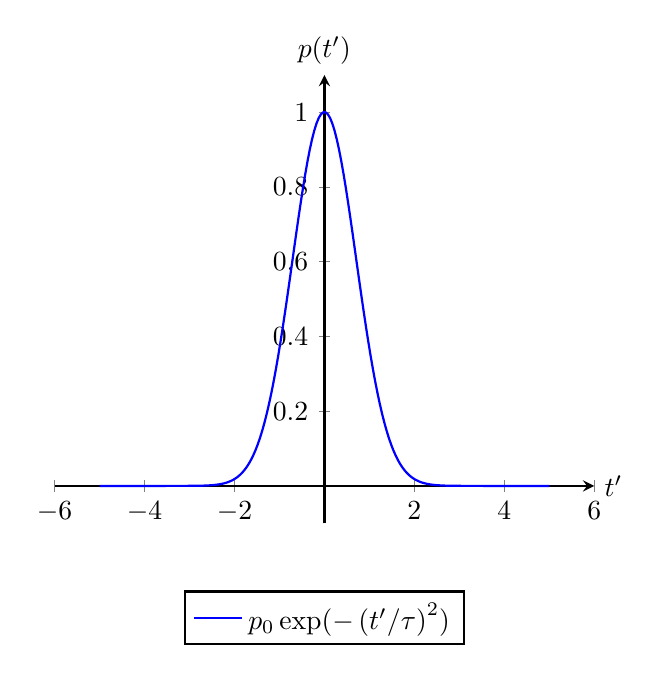
\begin{tikzpicture}
                    \begin{axis}[
                            axis lines=middle,
                            xlabel={$t'$},
                            ylabel={$p(t')$},
                            samples=200,
                            domain=-5:5,
                            thick,
                            enlargelimits,
                            legend style={at={(0.5,-0.15)}, anchor=north, legend columns=-1},
                            xlabel style={right},
                            ylabel style={above},
                        ]
                        \addplot[blue, thick] {exp(-x^2)};
                        \addlegendentry{$p_0 \exp(-\left({t'} / {\tau}\right)^2)$}
                    \end{axis}
                \end{tikzpicture}
            \end{center}

        \end{callout}
    \item[(b)] What is the radiation electric field at a location $\mathbf{r}$ (far from the dipole) and as a function of time?
        \begin{callout}{Solution:}

        Taking $\mathbf{E}$ and $\mathbf{B}$ and then the second derivative of the dipole moment,
        \begin{align*}
            \mathbf{\ddot{p}} = \frac{\partial^{2}\mathbf{p}}{\partial t'^{2}}&= \frac{\partial \mathbf{p}}{\partial t} \left( -\frac{ 2 t'}{\tau^{2}} \mathbf{p} (t') \right) 
            = p_{0} \left[ \left( \frac{t'}{\tau} \right)^{2} - 2 \right] \cdot \left( \frac{1}{\tau} \right)^{2} e^{- t'^2 / \tau^2} \mathbf{\hat{z}} \\
            \mathbf{\hat{r}} \times \mathbf{\ddot{p}} &= \frac{4t'^2-2\tau^2}{\tau^4} p_0 \exp\left(-\left(\frac{t'}{\tau}\right)^2\right) \hat{\boldsymbol{\phi}} \\
            \mathbf{\hat{r}} \times \mathbf{\hat{r}} \times \mathbf{\ddot{p}} &= \frac{4t'^2-2\tau^2}{\tau^4} p_0 \exp\left(-\left(\frac{t'}{\tau}\right)^2\right) \mathbf{\hat{z}} \\
        \end{align*}
        Therefore, we will have fields:
        \begin{align*}
            \mathbf{E}(\mathbf{r},t_{0}) &\approx \frac{\mu_{0}}{4 \pi r} [\mathbf{\hat{r}} \times (\mathbf{\hat{r}} \times \mathbf{\ddot{p}} )] 
            %= \frac{\mu_{0}}{4\pi r} \frac{4t'^2-2\tau^2}{\tau^4} p_0 \exp\left(-\left(\frac{t'}{\tau}\right)^2\right) \mathbf{\hat{z}} \\
            = \frac{\mu_{0} p_{0}}{4\pi r} \left[ \left( \frac{t'}{\tau} \right)^{2} - 2 \right] \cdot \left( \frac{1}{\tau} \right)^{2} e^{- t'^2 / \tau^2} \mathbf{\hat{z}} \\
            \mathbf{B}(\mathbf{r},t_{0}) &\approx -\frac{\mu_{0}}{4 \pi r c} [\mathbf{\hat{r}} \times \mathbf{\ddot{p}}] 
            %= - \frac{\mu_{0}}{4\pi r c} \frac{4t'^2-2\tau^2}{\tau^4} p_0 \exp\left(-\left(\frac{t'}{\tau}\right)^2\right) \hat{\boldsymbol{\phi}} \\
            = -\frac{\mu_{0} p_{0}}{4\pi r c} \left[ \left( \frac{t'}{\tau} \right)^{2} - 2 \right] \cdot \left( \frac{1}{\tau} \right)^{2} e^{- t'^2 / \tau^2} \mathbf{\hat{\phi}} \\
            \mathbf{S}(\mathbf{r}, t_{0}) &\approx \frac{\mu_{0}}{16\pi^{2}} [\ddot{\mathbf{p}}(t_{0})]^{2} \frac{\sin^{2} \theta}{r^{2}} \hat{r}
        \end{align*}

        \end{callout}
    \item[(c)] What is the power detected at $\mathbf{r}$ and as a function of time? Use spherical coordinates.
        \begin{callout}{Solution:}

            $$P(r, t) = \oint \mathbf{S}(\mathbf{r}, t) \,d \mathbf{a} = \frac{\mu_{0}}{6\pi c}\left( \ddot{p} \left( t - \frac{r}{c} \right) \right)^{2}$$

            Substituting in our ${\ddot{p}}$, 
            $$\boxed{P=\frac{\mu_{0}}{6\pi c}\left( p_{0} \left[ \left( \frac{t_0}{\tau} \right)^{2} - 2 \right] \cdot \left( \frac{1}{\tau} \right)^{2} e^{- t_0^2 / \tau^2} \mathbf{\hat{z}} \\ \right)^{2}}$$

            where $t_{0}= t- \frac{r}{c}$.

        \end{callout}
    \item[(d)] \textit{Qualitatively}, what would the Fourier transform of the electric field at $\mathbf{r}$ look like versus frequency? If you were designing a detector/receiver what is the rough frequency you would design it for?
        \begin{callout}{Solution:}

        The characteristic frequency is given by the fourier transform, and is roughly $1 / \tau$, so you would need electronics that can handle signals that oscillate at that frequency. If we had a nanosecond pulse, we'd be working with a gigahertz.

        \end{callout}
\end{itemize}
\end{homeworkProblem}
